\chapter{複雑系としての社会契約}
「倫理ある商取引ゲーム」において、倫理という限定合理性を仮定した上で商取引システムのインセンティブ設計を行えば、
プレイヤーの構成によっては不正が防止され、商取引契約の内容が果たされるようになることがわかった。
本章では、この商取引契約の内容に焦点を当て、これまで外部の強制執行力として存在が仮定されていた「商取引システム」を、
ある集団の成員が構成する複雑系の内部で自己組織化されたシステムとして再現する商取引契約の内容について提案し、
マルチエージェントシミュレーションによって、商取引システムが存在しない場合でも、社会契約が成立しうることを示す。

\section{本章の問題提起}
本章では先の章で扱った「倫理ある商取引ゲーム」において、外部の強制執行力として存在が仮定されていた「商取引システム」が存在しない場合でも、
プレイヤーの構成によって「商取引ゲーム」の不正を防止することが可能であるかという問いに取り組む。

\section{本章の仮説}
商取引システムが存在する場合に、商取引契約を履行させることが可能であるとする。
このとき、各プレイヤーが商取引システムと同様の役割を演じることができれば、
外部の強制執行力としての商取引システムが存在せずとも相互監視の元で商取引ゲームで不正を防止し続けることが可能となるだろう。

\section{提案手法}
先の仮説を検証するためには、
各プレイヤーが商取引システムの役割を正しく演じる商取引契約の内容を記述し、
その商取引契約の履行を約束する「商取引ゲーム」を繰り返した結果、
全てのプレイヤーが「商取引ゲーム」で不正を行えない状態になりうることを示す必要がある。

ここで、「商取引システム」とはどういったシステムであったかに立ち返ると、
「商取引システム」とは、各プレイヤーの初期の通貨保有量と保存された各時刻の商取引の記録から、
各プレイヤーの通貨保有量を一意に決定するシステムである。
それ故、初期の通貨保有量と保存された各時刻の商取引の記録が全てのプレイヤーで一致しているとき、
全てのプレイヤーが商取引システムが正しく動作しているといえる。

それを実現するためには、各プレイヤーが保存している過去の商取引の記録を互いに確認し合い、
差異が生じた場合に全てのプレイヤーに「失敗」を報告する商取引契約の内容を記述すればよい。

そこで、本章では下記のような「成員の振る舞い」を提案し、
先の仮説が成り立つことを検証する。

\subsection{成員の振る舞い}
  \begin{itemize}
    \item 事前の合意に基づいた全てのプレイヤーの人数$n$と各プレイヤーの初期の通貨保有量$b_i, ..., b_n$を定義する。
    \item 事前の合意に基づいた各プレイヤーが他の全てのプレイヤーと$seller$と$buyer$のそれぞれの役割で1度づつ「商取引ゲーム」を行う周期を定義する。(周期の長さは$ n * (n-1)$)
    \item 事前の合意に基づいた仕様に従った商取引システムを用意する。
    \item 事前の合意に基づいた商取引契約の内容を定義する。
    \item 時刻tにおいて、「時刻tにおける成員の振る舞い」を上から順に実行する。
    \item 商取引の記録とは、商取引が行われた時刻$t$と$seller$、$buyer$、結果、報告者からなる記録とする。
  \end{itemize}

\subsection{時刻tにおける成員の振る舞い}
  
\begin{description}
  % sellerとbuyerの決定
  \item[step 1] 現在時刻の$seller$と$buyer$を決定する。 
  % ビザンチン将軍問題の司令の再配布
  \item[step 2] 自身が$seller$ならば、時刻$\max\{0, t-n*(n-1)\}$から時刻$t$までの各時刻$k$について、
    保管されている商取引の記録のうち、時刻が$k$で報告者がその商取引の記録の$buyer$と一致するものを全て集め複製する。
    その複製された全ての商取引の記録に署名して$buyer$に送信する。
  % ビザンチン将軍問題の再配布された司令の受け取り
  \item[step 3] 自身が$buyer$ならば、$seller$から受け取った記録の署名を検証し、
    添付された全ての商取引の記録の報告者を$seller$に書き換えて保管する。
    $seller$からメッセージを受け取っていない場合、このstepでは何もしない。
  % 商取引システムの状態の決定
  \item[step 4] 自身が$buyer$ならば、時刻$\max\{0, t-2*n*(n-1)\}$から時刻$\max\{0, t-n*(n-1)\}$までの各時刻$k$について、
    保管されている商取引の記録のうち、時刻が$k$のものを集め、それらの結果が全て一致しているかを確認する。
    もし一致している場合、その一致した結果を商取引システムに報告された結果として入力する。
    一致しない場合、またはその時刻の商取引の記録が存在しない場合、報告された結果として自身の商取引システムに「失敗」を入力する。
  % 商取引の結果の決定
  \item[step 5] 自身が$buyer$ならば、商取引契約の結果を決定する。
  % ビザンチン将軍問題の司令
  \item[step 6] step5で決定した結果をもとに商取引の記録を作成し、署名して、全てのプレイヤーに送信する。
  % ビザンチン将軍問題の司令の受け取り
  \item[step 7] $buyer$から報告された商取引の記録を保管する。この際、記録の報告者は$buyer$とする。
    $buyer$から報告を受け取っていない場合、このstepでは何もしない。
\end{description}

\section{実験方法}
  ここでは「時刻tにおける成員の振る舞い」のstep 6が必ず遵守される状態を作り出せるかを確認するため、
  下記の「実験用の商取引契約」を合意された商取引契約として、
  これを履行する場合と履行しない場合で4種づつ、計8タイプのエージェントを用意する。
  この8タイプのエージェントから重複問わずランダムに選んだ8体のエージェントを用意し試行を実施する。
  これをタイプAのエージェントが0〜7体を占める場合について、それぞれ8000回づつ繰り返し、
  エージェントの構成とstep9で求まる「報告された成功率」と「真の成功率」を記録する。

  \subsection{実験用の商取引契約}
  $seller$が「成員の振る舞い」のstep6の通りに振る舞う対価として、$buyer$が通貨を1支払う商取引契約を結ぶ。
  $buyer$は$seller$がこの商取引を履行したかどうかを「step6の検証」によって確認することができる。

  \subsection{step6の検証}
  時刻$t$において、$buyer$は$seller$が「成員の振る舞い」のstep6を履行したかを下記の2つの検証で確かめることができる。
  検証1は全てのプレイヤーに同じ商取引の結果を送信したことを検証する方法であり、
  検証2は$buyer$に商取引の結果を送信したかを検証する方法である。
  
  \begin{description}
    % sellerがstep 6で全員に同じ司令を送っていたかの確認
    \item[検証1] 時刻$\max\{0, t-2*n*(n-1)\}$から時刻$\max\{0, t-n*(n-1)\}$までのうち、
      その時刻に行われた商取引の$buyer$が現在時刻の商取引の$seller$である各時刻$k$について、
      保管されている商取引の記録のうち、時刻が$k$のものを集め、
      その中に報告者が時刻$t$の商取引の$seller$が存在し、
      それらの結果が一致していることを確認する。
    % sellerがstep 6で自身に司令を送っていたかの確認
    \item[検証2] 時刻$\max\{0, t-2*n*(n-1)\}$から時刻$\max\{0, t-n*(n-1)\}$までのうち、
      その時刻に行われた商取引の$buyer$が現在時刻の商取引の$seller$である各時刻について、
      保管されている商取引の記録のうち、その時刻の商取引の記録を集めて、
      その中に報告者が現在時刻の商取引の$seller$である記録が存在するかを確認する。
  \end{description}

  
  \subsection{エージェントの種類}
    下記の8タイプのエージェントを用意する。下記に記述のない振る舞いに関しては「成員の振る舞い」に従う。
    \begin{itemize}
      \item[A] 完全に商取引契約を履行するエージェント
      \item[B] step5を無視して必ず「成功」を報告するエージェント
      \item[C] step5と逆の結果を報告するエージェント
      \item[D] step5を無視して必ず「失敗」を報告するエージェント
      \item[E] step6でタイプAにだけ結果を送らないエージェント
      \item[F] step6でタイプAにだけ結果を送らず、step5を無視して必ず「成功」を報告するエージェント
      \item[G] step6でタイプAにだけ結果を送らず、step5と逆の結果を報告するエージェント
      \item[H] step6でタイプAにだけ結果を送らず、step5を無視して必ず「失敗」を報告するエージェント
    \end{itemize}

  \subsection{試行}
    \begin{description}
      \item[step 1] 時刻tを0とする。
      \item[step 2] 各プレイヤーが互いにsellerとbuyerのそれぞれの役割で1度づつ商取引ゲームを行う順序を決定し、各エージェントが合意する。(順序の長さは56となる)
      \item[step 3] プレイヤー数は8、初期の通貨保有量は各プレイヤー8、商取引システムの仕様は前章の実験と同じものとし、各エージェントが合意する。
      \item[step 4] 時刻tを1進める。
      \item[step 5] 各エージェントはその特性に則って振る舞う。
      \item[step 6] 各エージェントの「商取引システム」において、時刻tの入力によって誰の通貨保有量も0未満にならない場合、報告された結果を記録する。
      \item[step 7] 各エージェントの「商取引システム」において、時刻tの入力によって誰の通貨保有量も0未満にならない場合、真の結果を記録する。
      \item[step 8] 時刻tが1120未満なら、step4に戻る。
      \item[step 9] 各エージェントの「商取引システム」において、過去56回分のstep5と6で記録された結果を集計し、それぞれ「報告された成功率」と「真の成功率」を求める。
    \end{description}

\section{評価}
% 先の実験の結果、「報告された成功率」と「真の成功率」の両方が100\%になった場合を「不正防止の成功」とし、
% 誠実なエージェント(タイプA)の数と「不正防止の成功」に至った割合をプロットしたものが、図\ref{ethical-game-001}である。
% (エージェント数8の場合は、エージェントの組み合わせが1通りしか存在しないため、個別に試行を行い結果を集計している。)
% 誠実なエージェントの数が0体の場合であっても不正が防止される構成が存在し、
% 6体以上の場合はサンプリングした全ての構成で不正の防止が成功していた。

サンプリングした結果を元に、タイプAのエージェントと自己組織化が成功した割合をプロットすると、
図\ref{compex-system-002}のようになる。この図から、誠実なプレイヤーが6人以上の場合は全てのサンプルで自己組織化に成功していることがわかる。

\begin{figure}[h]
  \begin{tabular}{cc}
    \begin{minipage}[t]{1\hsize}
      \centering
      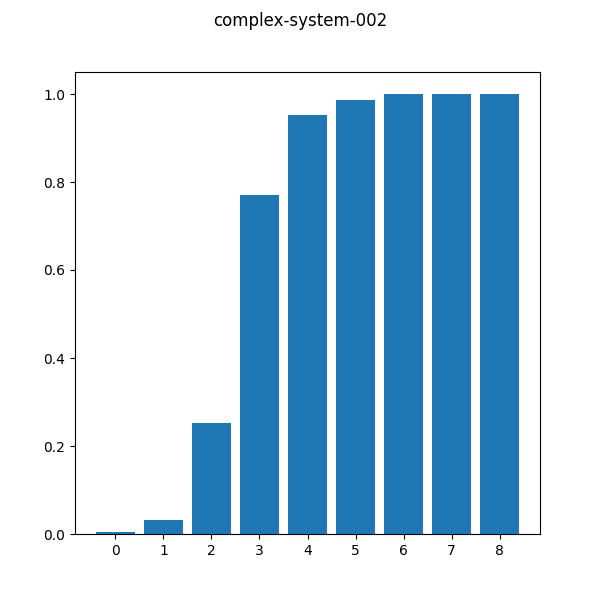
\includegraphics[keepaspectratio, width=1\linewidth]{./05_complex-system/complex-system-002.png}
      \caption{誠実なエージェントの数と自己組織化に成功した割合}
      \label{compex-system-002}
    \end{minipage}
  \end{tabular}
\end{figure}
